\begin{titlepage}
  \begin{tikzpicture}[remember picture, overlay]
    % Logo dan latar belakang
    \node[anchor=north west, inner sep=0pt] at ([xshift=.18\textwidth, yshift=-.1\textwidth] current page.north west){
      
\includegraphics[width=.3\paperwidth]{../figures/images/logo_universitas.png}
    };

    \node[anchor=north west, inner sep=0pt, opacity=.12] at (current page.north west){
      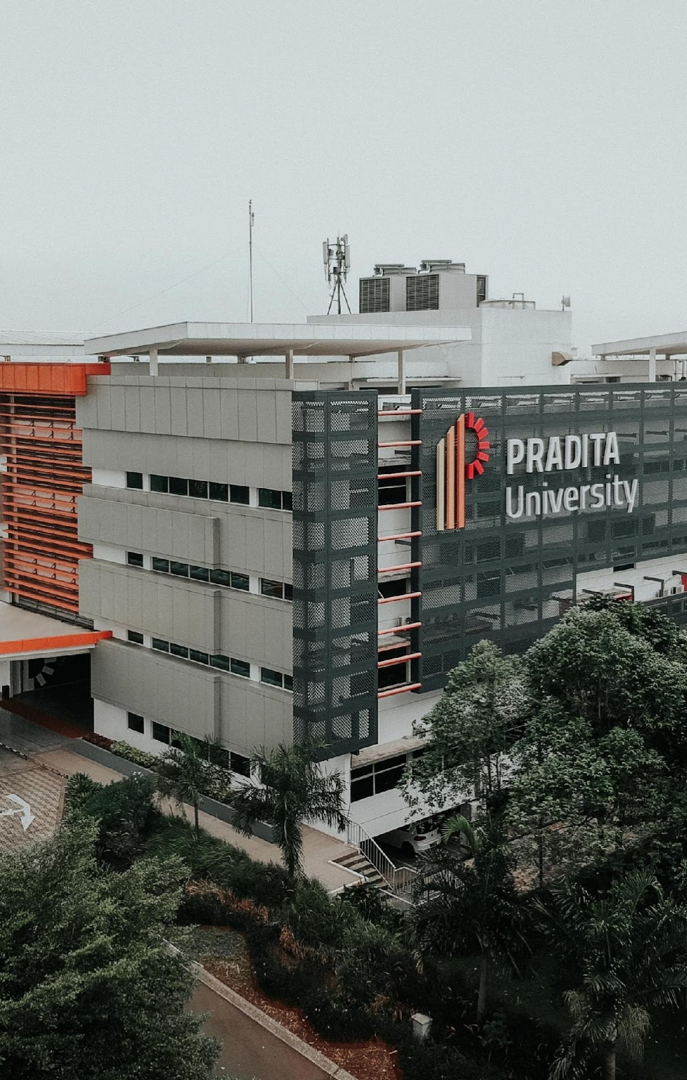
\includegraphics[width=\paperwidth]{../figures/images/building.png}
    };

    % Judul
    \node[anchor=center] at ([yshift=.1\textheight]current page.center) {
      \begin{minipage}{\textwidth}

        {\fontsize{34}{41}\selectfont \textcolor{praditagreen}{
        \textbf{Dasar Pemrograman\\[10pt]
            dengan GenAI Terarah
        }}}\\[.05\textheight]
        {\LARGE \textbf{Alfa Yohannis, Ariya Panna}}\\[0.02\textheight]
        {\large \today}
      \end{minipage}
    };

    % Panel bawah
    \node[anchor=south west] at (
    current page.south west) {
      \begin{tikzpicture}[remember picture, overlay]
        \node[anchor=south west, fill=praditagreen, text=white, minimum width=\paperwidth, minimum height=.14\textheight, align=center, font=\Huge\bfseries] at (-.15,-.15) {
          Program Studi Informatika\\
          Universitas Pradita
        };
      \end{tikzpicture}
    };
  \end{tikzpicture}
\end{titlepage}
